% ==============================================================================
% TCC - Nome do Aluno
% Capítulo 2 - Referencial Teórico
% ==============================================================================
\chapter{Algoritmo de Dijkstra}
\label{sec-dijkstra}

\section{O Algoritmo}
\label{sec-dijkstra-algoritmo}
O algoritmo de Dijkstra foi proposto por Edgar W. Dijkstra em 1959 \cite{dijkstra1959note}. Ele tem por objetivo definir o menor caminho partindo do vértice origem $v_{s}$ e chegando a todos os demais vértices $v_{i}$ do grafo $G = (V,E)$. Para garantir a viabilidade do algoritmo, assume-se que todos os pesos $w( u, v )$ sejam maiores ou iguais a zero para toda aresta $E$ do grafo $G$ \cite{cormen2009introduction}.

A seguir é apresentado o pseudocódigo do algoritmo conforme descrito em \citeonline{drozdek2012data}.
%\begin{verbatim}
%CÓDIGO AQUI
%\end{verbatim}

\begin{lstlisting}[ mathescape, label=lst-dijkstra-codigo, caption=Algoritmo de Dijkstra., float=htpb]
DijkstraAlgorithm(weighted simple digraph, vertex first)
	for all vertices v
		currDist(v) = $\infty$;
	currDist(first) = 0;
	toBeChecked = all vertices;
	while toBeChecked is not empty
		v = a vertex in toBeChecked with minimal currDist(v);
		remove v from toBeChecked;
		for all vertices u adjacent to v and in toBeChecked
			if currDist( u ) > currDist( v ) + weight( edge(vu) )
				currDist( u ) = currDist( v ) + weight( edge(vu) );
				predecessor( u ) = v;
\end{lstlisting}

%\begin{verbatim}
%DijkstraAlgorithm(weighted simple digraph, vertex first)
%	for all vertices v
%	currDist(v) = infinite;
%	currDist(first) = 0;
%	toBeChecked = all vertices;
%	while toBeChecked is not empty
%		v = a vertex in toBeChecked with minimal currDist(v);
%		remove v from toBeChecked;
%		for all vertices u adjacent to v and in toBeChecked
%		if currDist( u ) > currDist( v ) + weight( edge(vu) )
%			currDist( u ) = currDist( v ) + weight( edge(vu) );
%			predecessor( u ) = v;
%\end{verbatim}

O algoritmo inicia atribuindo o valor inicial de cada distância de cada vértice do grafo igual a $\infty$, com exceção do vértice inicial $v_{s}$ que será iniciado por 0. Em seguida todos os vértices são adicionados ao conjunto dos "toBeChecked" ("aSeremChecados"). Feito isso, inicia-se o processo iterativo: seleciona-se o vértice $v$ de menor custo que esteja dentro do conjunto "toBeChecked", retira-se ele do conjunto e a partir dele, para cada vértice adjacente $u$ de $v$, verifica-se se a distância atual calculada de $u$ é maior do que a distância calculada de $v$ mais o valor referente ao peso da aresta de $v$ e $u$ (origem em $v$). Caso seja verdade, a distância atual de $u$ é substituída pela soma da distância atual de $v$ mais o peso da aresta de $v$ e $u$ (este valor corresponde à distância do vértice de origem $v_{s}$ até $u$), além de definir o antecessor $u$ como $v$. Repete-se o passo iterativo até que o conjunto "toBeChecked" esteja vazio\footnote{Em linguagens de programação, é costume substituir o valor $\infty$ pelo maior número representativo do tipo da variável selecionado para representar a distância. Por exemplo na linguagem C, caso se utilize o valor int (inteiro) para representar a distância, a atribuição inicial será dado pela constante INT\underline{\space}MAX  definida pela biblioteca "limits.h", que representa o maior valor numérico representado por esse tipo de variável.}.
\newpage
Ao final do algoritmo, teremos o conjunto de predecessores de cada vértice do grafo, e a partir deste, poderemos definir a rota para qualquer vértice do grafo partindo de $v_{s}$. O caminho retornado é garantidamente ótimo como mostra \citeonline{cormen2009introduction}.

A figura \ref{fig-dijkstra-algoritmo-grafo} mostra um exemplo de aplicação do algoritmo a um grafo.

\begin{figure}[H]
\centering
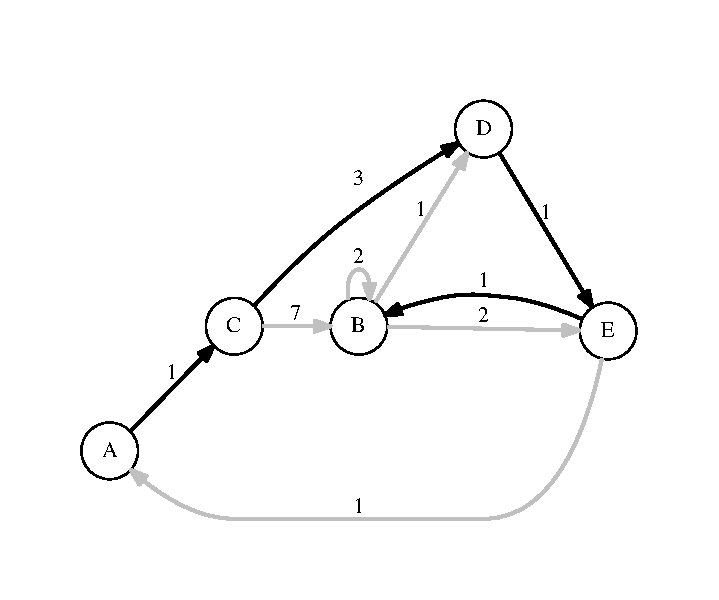
\includegraphics[width=1.\textwidth]{figuras/grafo-dijkstra} 
\caption{Aplicação do algoritmo de Dijkstra tendo o vértice "A" como origem. As arestas pintadas de preto correspondem a rota calculada a todos os demais vértices.}
\label{fig-dijkstra-algoritmo-grafo}
\end{figure}

Inicialmente a distância do vértice "A" é atribuído como zero enquanto de todos os demais é atribuído como infinito $\infty$. Inicia-se o processo iterativo a partir de "A" que explora os seus vértices adjacentes, que neste caso só tem um que é o vértice "C". A distância de "C" é calculada como o valor da distância de "A" mais o peso da aresta "AC" (que é igual a 1), e o vértice que é atribuído como antecessor de "C" é "A". Em seguida é escolhido o vértice cuja a distância seja a menor dentro do conjunto "toBeChecked" que neste caso é o próprio "C". Do vértice "C" explora-se os vértices adjacentes dele "D" e "B". Suas respectivas distâncias são atribuídas como a distância de "C" mais o peso de suas respectivas arestas (currDist( B ) = 7 + 1; currDist( D ) = 3 + 1), além de atribuir como "C" os seus respectivos vértices antecessores. Disso novamente, escolhe-se o vértice com menor distância em "toBeChecked" que neste caso será o D (currDist( D ) = 4 < currDist( C ) = 8). De "D" é explorado seu vértice adjacente "E" que é atribuído seu valor currDist( E ) como sendo 5 (3 + 1 + 1) e seu vértice antecessor como "D". Busca-se novamente o menor valor dos vértices em "toBeChecked" que neste caso será o "E" (currDist( E ) = 5 < currDist( B ) = 8). Dele explora-se os seus vértices adjacentes "B" e "A". O único valor da distância que é alterado é o de "B" pois o caminho vindo por "E" (A->C->D->E = 1 + 3 + 1 + 1) é menor do que o vindo por "C"  (A->C->B = 1 + 7). Finalmente, o vértice "B" é explorado, mas nenhum de seus vértices adjacentes tem o valor de sua distância alterado pois o menor caminho para eles já foi encontrado.

\section{Versões do Algoritmo implementadas e suas Estrutura de Dados}
\label{sec-dijkstra-versoes}
Neste projeto de graduação foram implementadas três versões do algoritmo de Dijkstra usando estruturas de dados diversas.

As versões implementadas são o Dijkstra Canônico (descrito a seguir), Dijkstra Heap Binário (subseção \ref{sec-dijkstra-versoes-heap}) e Dijkstra Heap de Fibonacci (subseção \ref{sec-dijkstra-versoes-fibonacci}), todas baseadas em \citeonline{cormen2009introduction, drozdek2012data}.

Para a versão Dijkstra Canônico o algoritmo utiliza um vetor para armazenar as distâncias calculadas pelo algoritmo (o indíce dos vértices correspondem ao indíce do vetor em que são armazenados), e a cada passo iterativo (conforme demonstrado pelo algoritmo na seção \ref{sec-dijkstra-algoritmo}), uma busca linear é realizada para determinar o vértice (fora do conjunto "toBeChecked") cuja distância é menor dentre todas as outras. A complexidade para esse caso é $O(|V^{2}|)$ \cite{drozdek2012data}.

\subsection{Dijkstra Heap Binário}
\label{sec-dijkstra-versoes-heap}
Para esta implementação, será utilizada a estrutura de dados heap binária mínima como fila de prioridade. Heaps binárias podem ser descritas como árvores binárias que possuem as seguintes propriedades \cite{drozdek2012data}:
\begin{enumerate}
 \item O valor de cada nodo não é maior do que os valores guardados em cada um de seus filhos.
 \item A árvore é perfeitamente balanceada, e as folhas no último nível estão todas posicionadas mais a esquerda.
\end{enumerate}

Um exemplo de estrutura Heap Binário representada tanto como árvore como vetor pode ser visualizado nas figuras \ref{fig-dijkstra-heapbinario} e \ref{fig-dijkstra-heapvetor} respectivamente.

\begin{figure}[H]
\centering
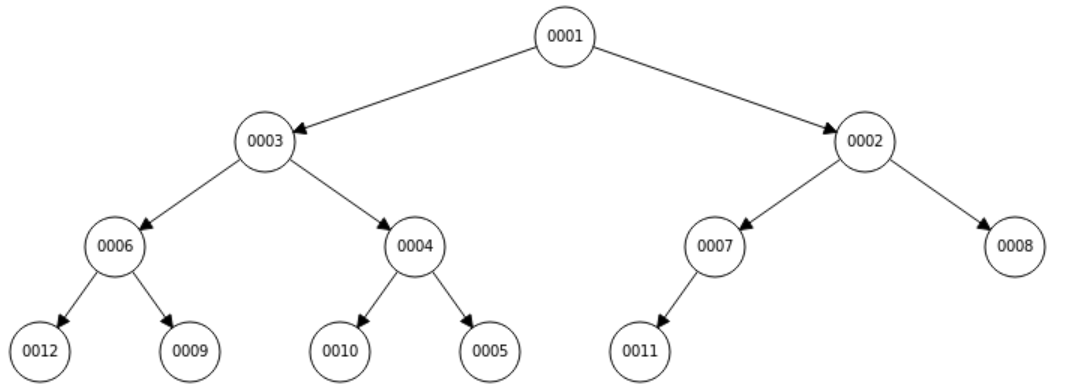
\includegraphics[width=.95\textwidth]{figuras/Heap} 
\caption{Exemplo de Heap Binário representado como árvore.}
\label{fig-dijkstra-heapbinario}
\end{figure}

\begin{figure}[H]
\centering
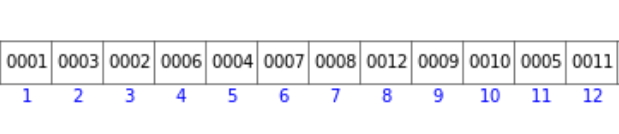
\includegraphics[width=.60\textwidth]{figuras/Heap-vetor}
\caption{Representação do Heap Binário da figura \ref{fig-dijkstra-heapbinario} como vetor.}
\label{fig-dijkstra-heapvetor}
\end{figure}

A disposição dos elementos da árvore no vetor segue as seguintes relações entre nós pai, filho-direita e filho-esquerda:
%\begin{equation}
%Pai(i): \lfloor i/2 \rfloor
%\end{equation}
%\begin{equation}
%Filho-esquerda(i): 2*i
%\end{equation}
%\begin{equation}
%Filho-direita(i): 2*i+1
%\end{equation}
\begin{description}
\item[pai($i$):] $\lfloor i/2 \rfloor$
\item[filho-esquerda($i$):] $2*i$
\item[filho-direita($i$):] $2*i+1$
\end{description}
Onde $i \in \mathbb{N}$ e $i \in [1, n]$, sendo que $i$ representa o índice do elemento no vetor e $n$ o número de elementos da árvore.

 Para efeito de exemplo (observe as figuras \ref{fig-dijkstra-heapbinario} e \ref{fig-dijkstra-heapvetor} para constatação), o nó que está contido na posição 4 do vetor possui como pai o nó de posição 2 ($\lfloor 4 / 2 \rfloor = 2$), tem como filho da esquerda o nó de posição 8 ($2*4 = 8$) e filho da direita o nó de posição 9 ($2*4+1 = 9$).

%\begin{equation}
%\forall i, i \in \mathbb{N} [1,n]
%\end{equation}

A vantagem de se usar essa estrutura de dados reside no fato de suas operações de inserção, extração de mínimo e reconstrução da heap possuírem complexidade de $O(\lg n)$. Por consequência, o tempo computacional para este caso é de $O(|E| \lg |V|)$ \cite{cormen2009introduction}.

\subsection{Dijkstra Heap de Fibonacci}
\label{sec-dijkstra-versoes-fibonacci}
A Heap de Fibonacci consiste de uma coleção de árvores que seguem a regra de árvore heap mínima, ou seja, os nós pais são maiores ou iguais aos nós filhos. Os nós raízes de cada árvore são interligados por uma lista circular duplamente encadeada. Um ponteiro chamado "raiz mínima" aponta para o nó de menor valor.

Sua característica é que operações de adição são executadas de uma maneira "preguiçosa", não procurando criar uma forma para as árvores (como por exemplo, deixá-la balanceada), apenas as adicionando à lista principal de raízes. Por consequência, operações de inserção possuem tempo computacional $O(1)$ \cite{cormen2009introduction}.

\begin{figure}[H]
\centering
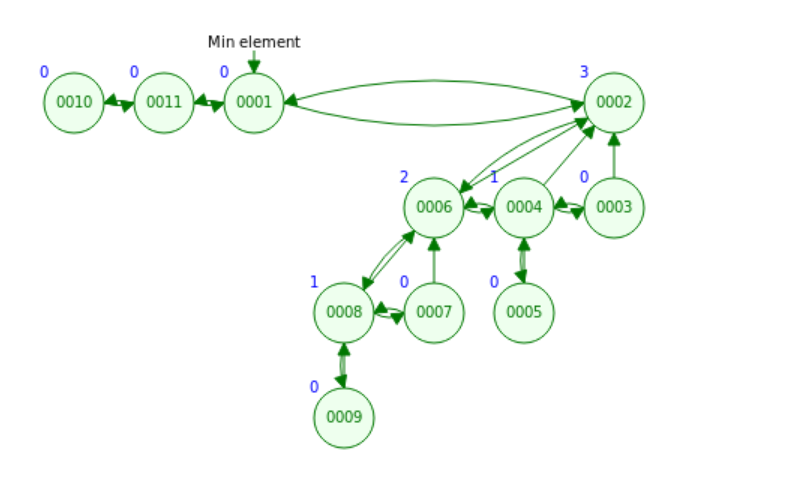
\includegraphics[width=.54\textwidth]{figuras/fibonacci-heap1} 
\caption{Exemplo de Heap de Fibonacci (os números no canto superior esquerdo de cada nodo correspondem ao grau de cada um, ou seja, o número de filhos).}
\label{fig-dijkstra-heapfibonacci1}
\end{figure}

Para operações de extração de mínimo o tempo computacional é mais custoso. Isso é devido ao fato de que quando o mínimo é retirado, a heap precisa ser reorganizada de forma que sua propriedade principal não seja violada e o um novo mínimo seja determinado. Para isso a operação de extração de mínimo se dá em três etapas. Primeiro é retirado o mínimo da heap (se caso o mínimo possua nós filhos, eles são colocados na lista principal de raízes) e o seu vizinho é assimilado como o novo mínimo provisório. Agora precisamos definir quem é o novo mínimo e para isso teremos que verificar todos os demais nós raízes. Com o intuito de diminuir o número de nós raízes é que o segundo passo é aplicado.  Ele consiste em lincar raízes com o mesmo número de grau (grau corresponde ao número de filhos que cada nodo possui) e para cada par de nodos licandos, verifica-se qual dos dois é menor. O que for o menor será o nodo pai e outro por consequência será o nodo filho. Após a lincagem de todos os nodos com mesmo número de grau, uma busca linear é realizada para se determinar o menor elemento entre os nodos raízes restantes\footnote{Para otimizar a busca de nodos com o mesmo número de grau é utilizado um vetor auxiliar de tamanho mínimo ao maior grau de um nodo da estrutura. Esse vetor contém ponteiros para os nodos e a posição desse nodo no ponteiro corresponde ao grau do nodo. Por exemplo, se um nodo possui grau 3, ele ocupará a posição de número 3 no vetor. Quando um nodo da lista é referenciado na posição que já está ocupado, o processo de lincagem é feito conforme descrito.}. O tempo computacional para a extração de mínimo é $O(\lg n)$ \cite{cormen2009introduction}.

%\footnote{Para otimizar a busca de nodos com o mesmo número de grau é utilizado um vetor auxiliar de tamanho mínimo ao maior grau de um nodo da estrutura. Esse vetor contém ponteiros para os nodos e a posição desse nodo no ponteiro corresponde ao grau do nodo. Por exemplo, se um nodo possui grau 3, ele ocupará a posição de número 3 no vetor. Quando um nodo da lista é referenciado na posição que já está ocupado, o processo de lincagem é feito conforme descrito.}

\begin{figure}[H]
\centering
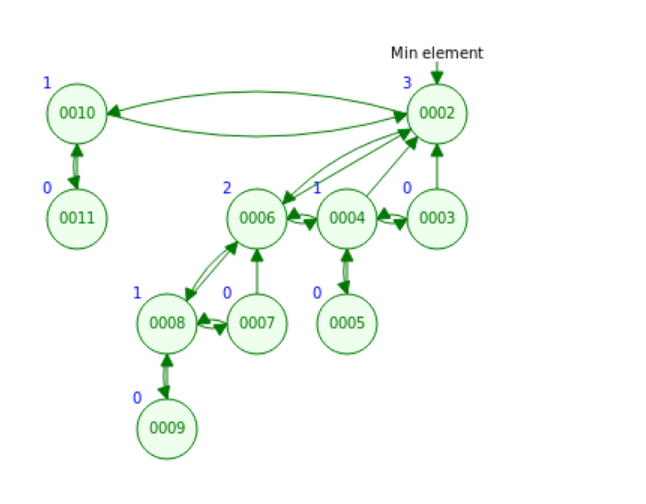
\includegraphics[width=.54\textwidth]{figuras/fibonacci-heap2} 
\caption{Heap de Fibonacci da figura \ref{fig-dijkstra-heapfibonacci1} após a operação de extração de mínimo.}
\label{fig-dijkstra-heapfibonacci2}
\end{figure}


Finalmente para a operação de mudança de chave de um determinado nodo, e após a mudança realizada em tempo constante ($O(1)$), é verificado se a propriedade heap foi violada. Se caso sim, esse nodo é cortado de seu nodo pai e colocado junto a lista principal. Se o pai não pertencer a lista de nodos raízes, ele é "marcado" ("pintado") e caso já estivesse "marcado" ele também é cortado e seu pai é "marcado". Esse processo continua subindo até encontrarmos um nodo pai "não marcado" ou um nodo raiz. Após esse processo recursivo ter terminado, verifica-se se nodo modificado inicialmente é menor do que o nodo mínimo atual. Se caso sim, o novo nodo mínimo é o modificado. O tempo computacional é $O(1)$ \cite{cormen2009introduction}.

Por consequência, o tempo computacional aplicado para o algoritmo de Dijkstra é de $O(|V|\lg |V| + |E|)$ \cite{cormen2009introduction}.